\section{Schematy różnicowe}
\subsection{Definicja}

MRS opiera się na zastąpieniu pochodnych występująych w równaniach różniczkowych poprzez formuły zwane \textbf{schematami różnicowymi}. 

Aproksymacja pochodnej polega na rozwiązywaniu w efektywny sposób równań rózniczkowych zwyczajnych i cząstkowych, gdzie równania te dane są poprzez formuły zawierające nieznaną funkcję, którą chcemy wyznaczyć oraz pochodne dowolnych rzędów, a także stałe i znane funkcje.

Załóżmy, że funkcja $\textbf{f}$ jest różniczkowalna, co oznacza, że pochodna $f'(x_{0})$ jest zdefiniowana i ograniczona w pewnym otoczeniu punktu $x_{0}$.

Wprowadźmy trzy podstawowe schematy różnicowe w celu aproksymacji wartości pochodnej $f'(x_{0})$:

$\bullet$ Schemat \textit{w tył} (backward approximation scheme) 

$$f'(x_{0})\approx D_{-}f(x_{0})=\frac{f(x_{0})-f(x_{0}-h)}{h}$$

$\bullet$ Schemat \textit{w przód} (forward approximation scheme) 

$$f'(x_{0})\approx D_{+}f(x_{0})=\frac{f(x_{0}+h)-f(x_{0})}{h}$$

Obie formuły dają aproksymację rzędu pierwszego, co oznacza, że błąd jest proporcjonalny do wielkości h.

$\bullet$ Schemat \textit{centralny} (central approximation scheme) 

$$f'(x_{0})\approx D_{c}f(x_{0})=\frac{f(x_{0}+h)-f(x_{0}-h)}{2h} = \frac{1}{2}(D_{+}f(x_{0})+D_{-}f(x_{0}))$$

Schemat centralny jest rzędu drugiego, a więc $Error \sim h^{2}$.

	\subsection{Cel ćwiczenia}
Dla wybranej funkcji $f$ mieliśmy użyć schematów różnicowych w celu aproksymacji wartości jej pochodnej, pierwszej oraz drugiej.

Wybraliśmy funkcję $sinus$ w punkcie $x_{0} = 0.3$.

Analitycznie obliczyliśmy pierwszą oraz drugą pochodną w obranym punkcie. Otrzymaliśmy:

$$sin'(0.3)=0.9553$$
$$sin''(0.3)=-0,2955$$

Następnie przystąpiliśmy do obliczeń numerycznych przy wykorzystaniu zaprezentowanych schematów różnicowych.
\newpage
\subsection{Wykresy}
\vspace{0.3cm}
Błędy oznaczone kolorem czerwonym nie były istotne podczas tworzenia wykresu, zostały one pominięte.

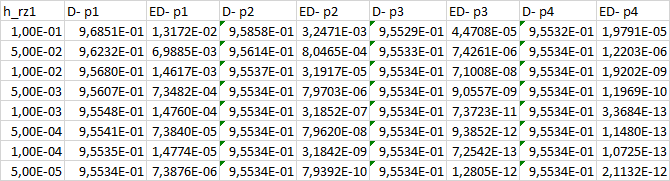
\includegraphics{Lab2/charts/rz1_log_Db_dane.png}

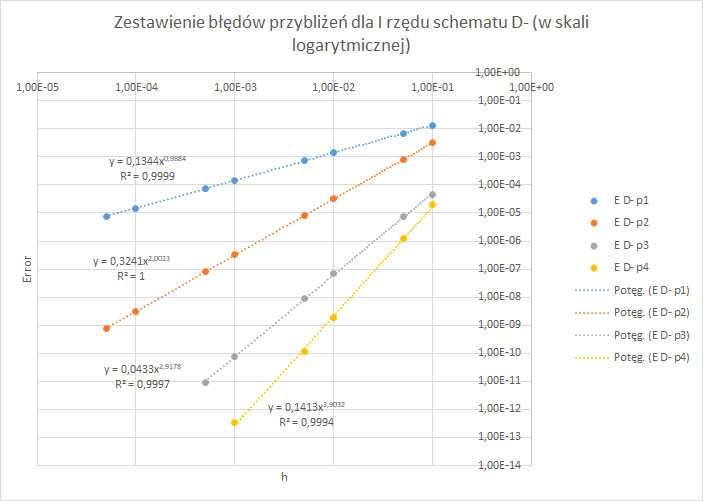
\includegraphics{Lab2/charts/rz1_log_Db.png} 
\newpage

Błędy oznaczone kolorem czerwonym nie były istotne podczas tworzenia wykresu, zostały one pominięte.

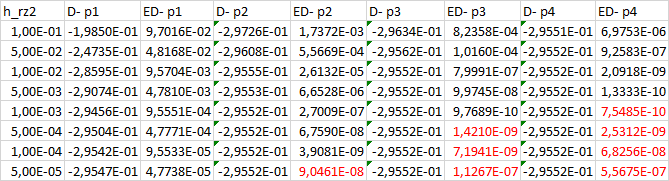
\includegraphics{Lab2/charts/rz2_log_Db_dane.png}

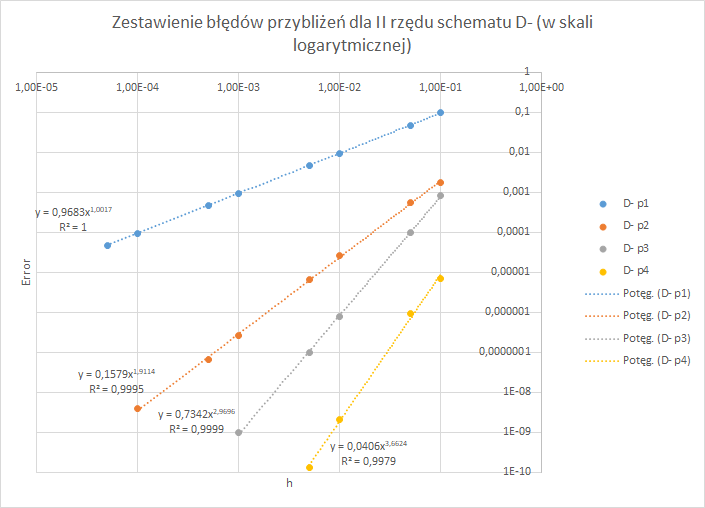
\includegraphics{Lab2/charts/rz2_log_Db.png}
\newpage

Błędy oznaczone kolorem czerwonym nie były istotne podczas tworzenia wykresu, zostały one pominięte.

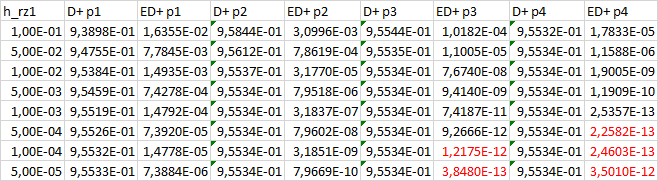
\includegraphics{Lab2/charts/rz1_log_Df_dane.png}

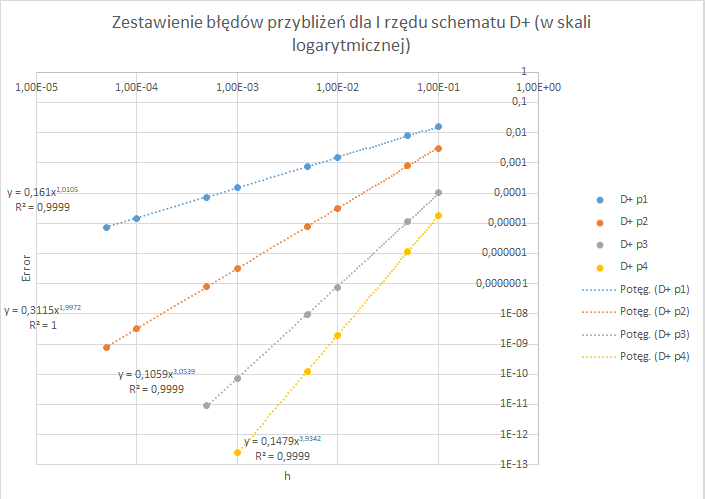
\includegraphics{Lab2/charts/rz1_log_Df.png}
\newpage

Błędy oznaczone kolorem czerwonym nie były istotne podczas tworzenia wykresu, zostały one pominięte.

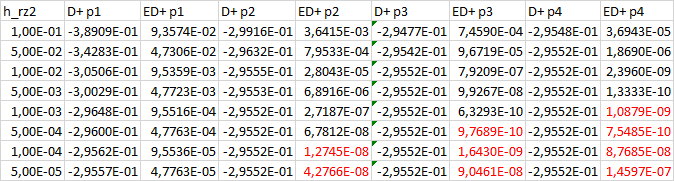
\includegraphics{Lab2/charts/rz2_log_Df_dane.png}

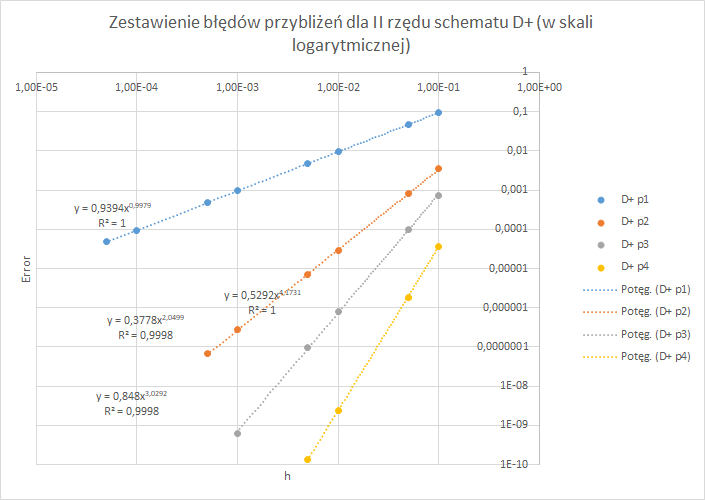
\includegraphics{Lab2/charts/rz2_log_Df.png}
\newpage

Błędy oznaczone kolorem czerwonym nie były istotne podczas tworzenia wykresu, zostały one pominięte.

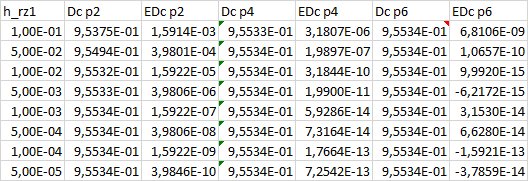
\includegraphics{Lab2/charts/rz1_log_Dc_dane.png}

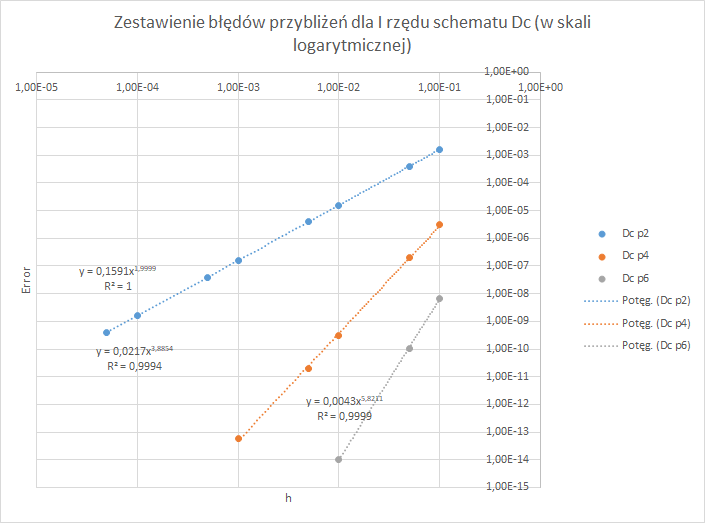
\includegraphics{Lab2/charts/rz1_log_Dc.png}
\newpage

Błędy oznaczone kolorem czerwonym nie były istotne podczas tworzenia wykresu, zostały one pominięte.

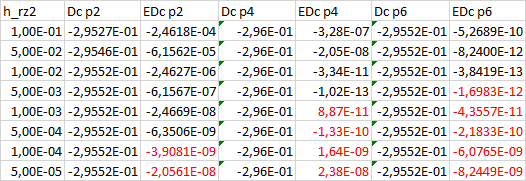
\includegraphics{Lab2/charts/rz2_log_Dc_dane.png}

Zestawienie błędów przybliżeń dla II rzędu schematu Dc na wykresie log-log nie jest możliwe. 

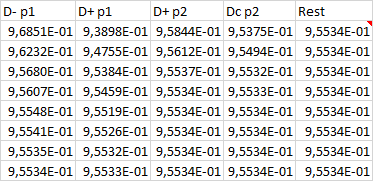
\includegraphics{Lab2/charts/rz1_log_e_dane.png}

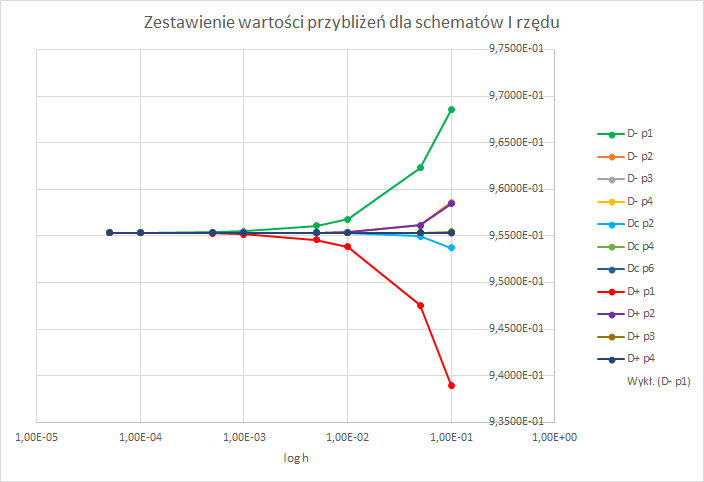
\includegraphics{Lab2/charts/rz1_log_e.png}
\newpage


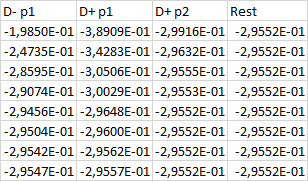
\includegraphics{Lab2/charts/rz2_log_e_dane.png}

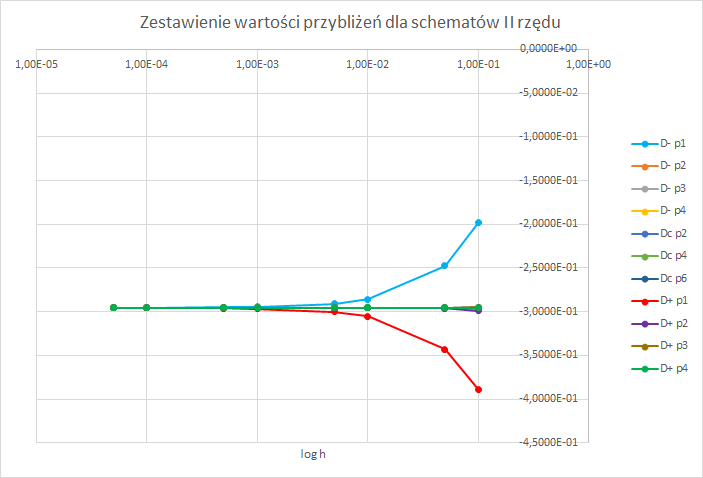
\includegraphics{Lab2/charts/rz2_log_e.png}
\newpage


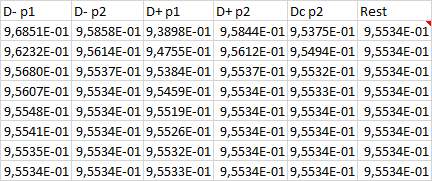
\includegraphics{Lab2/charts/rz1_e_dane.png}

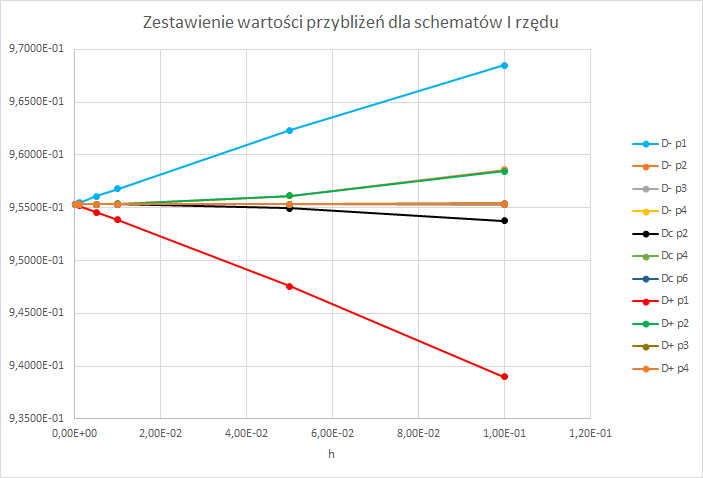
\includegraphics{Lab2/charts/rz1_e.png}
\newpage


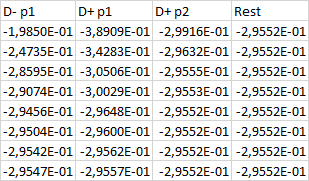
\includegraphics{Lab2/charts/rz2_e_dane.png}

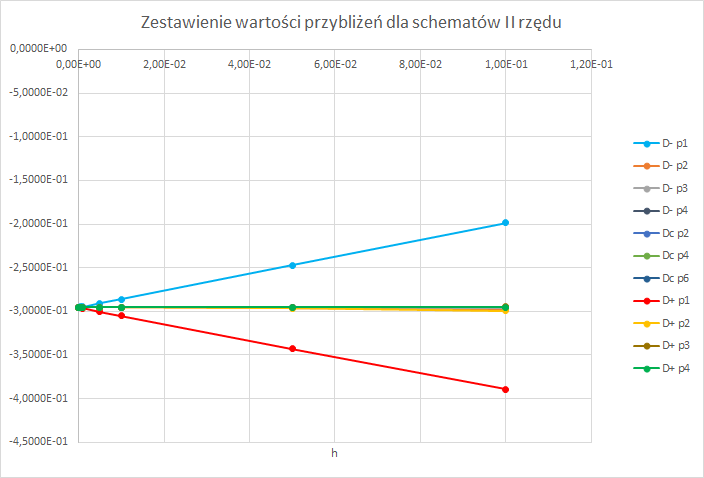
\includegraphics{Lab2/charts/rz2_e.png}

\subsection{Zadanie dodatkowe - Współczynniki}
Ponadto wyznaczyliśmy współczynniki dla:

$1)\hspace{1mm}Df(x_{0}) \leftarrow f(x_{0}), f(x_{0}-h), f(x_{0}-3h) $

$2)\hspace{1mm}Df(x_{0}) \leftarrow f(x_{0}-h), f(x_{0}), f(x_{0}+2h), f(x_{0}+3h) $

$3)\hspace{1mm}D^2f(x_{0}) \leftarrow f(x_{0}-2h), f(x_{0}-h), f(x_{0}), f(x_{0}+h) $
\vspace{0.3cm}

Aby rozwiązać ten problem użyliśmy rozwinięcie w szereg Taylora.

Przykładowe rozwiązanie prezentujemy dla pierwszego przykładu, kolejne zostały rozwiązane analogicznie.

\vspace{0,5cm}

$Df(x_{0}) = a \cdot f(x_{0}) + b \cdot f(x_{0}-h) + c \cdot f(x_{0}-3h) $

$f(x_{0}-h) = f(x_{0}) - \frac{f'(x_{0})}{1!}h + \frac{f''(x_{0})}{2!}h^2 + O(h^3)$

$f(x_{0}-3h) = f(x_{0}) - \frac{f'(x_{0})}{1!}3h + \frac{f''(x_{0})}{2!}9h^2 + O(h^3)$

$Df(x_{0}) = f(x_{0}) \cdot (a+b+c) + f'(x_{0}) \cdot (-bh-3ch) + f''(x_{0}) \cdot (\dfrac{bh^2}{2} + \dfrac{9ch^2}{2}) $

Teraz rozwiązujemy poniższy układ równań w celu wyznaczenia współczynników a, b oraz c.

\[
\begin{cases}
\vspace{0.1cm} 
\hspace{0,1cm}a+b+c=0 \\
\vspace{0.1cm}
\hspace{0,1cm}-bh-3ch=1 \\
\hspace{0,1cm}\dfrac{bh^2}{2} + \dfrac{9ch^2}{2}=0
\end{cases}
\]

Otrzymujemy:

Rozwiązanie zadania 1.

\[
\begin{cases}
\vspace{0.2cm} 
\hspace{0,1cm}a=\dfrac{4}{3h} \\
\vspace{0.2cm}
\hspace{0,1cm}b=-\dfrac{3}{2h} \\
\hspace{0,1cm}c=\dfrac{1}{6h}
\end{cases}
\]

Rozwiązanie zadania 2.

\[
\begin{cases}
\vspace{0.2cm} 
\hspace{0,1cm}a=\dfrac{1}{6h} \\
\vspace{0.2cm}
\hspace{0,1cm}b=-\dfrac{1}{2h} \\
\vspace{0.2cm}
\hspace{0,1cm}c=\dfrac{1}{2h} \\
\vspace{0.2cm}
\hspace{0,1cm}d=-\dfrac{1}{6h}
\end{cases}
\]

Rozwiązanie zadania 3.

\[
\begin{cases}
\vspace{0.2cm} 
\hspace{0,1cm}a=-\dfrac{2}{h^2} \\
\vspace{0.2cm}
\hspace{0,1cm}b=0 \\
\vspace{0.2cm}
\hspace{0,1cm}c=\dfrac{1}{h^2} \\
\vspace{0.2cm}
\hspace{0,1cm}d=\dfrac{1}{h^2}
\end{cases}
\]

Następnie przystąpiliśmy do obliczeń numerycznych wykorzystując trzy powyższe schematy.

\newpage

Błędy oznaczone kolorem czerwonym nie były istotne podczas tworzenia wykresu, zostały one pominięte.

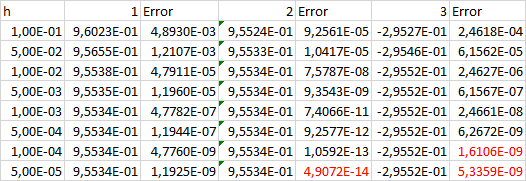
\includegraphics{Lab2/charts/wsp_log_dane.png}

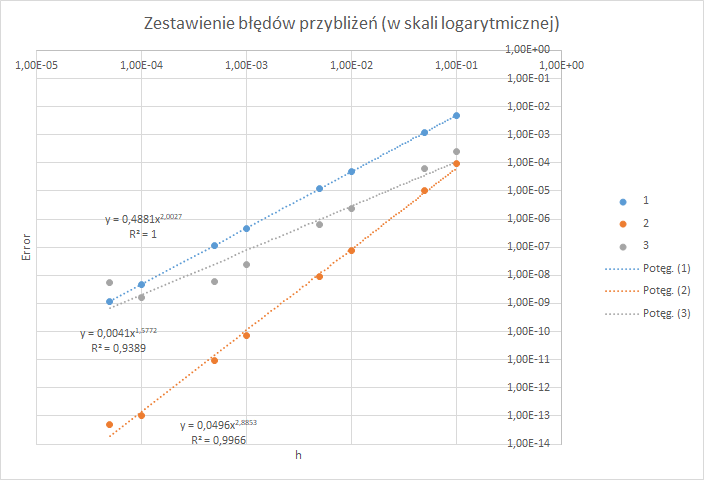
\includegraphics{Lab2/charts/wsp_log.png}
\newpage

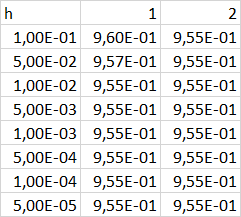
\includegraphics{Lab2/charts/wsp_log_e_dane.png}

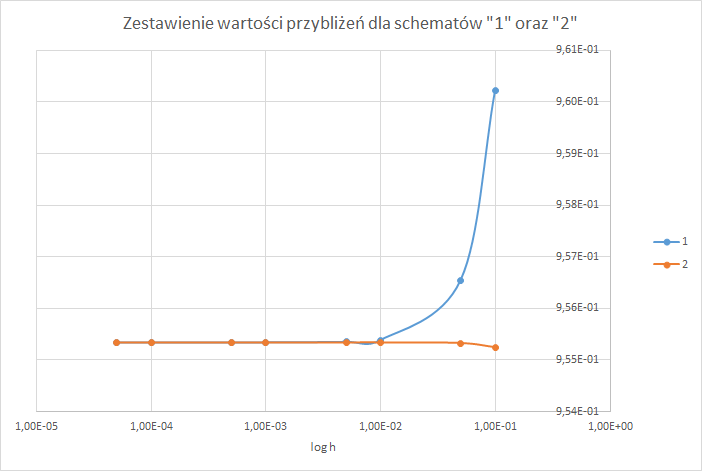
\includegraphics{Lab2/charts/wsp_log_e.png}
\newpage

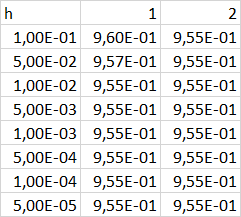
\includegraphics{Lab2/charts/wsp_log_e_dane.png}

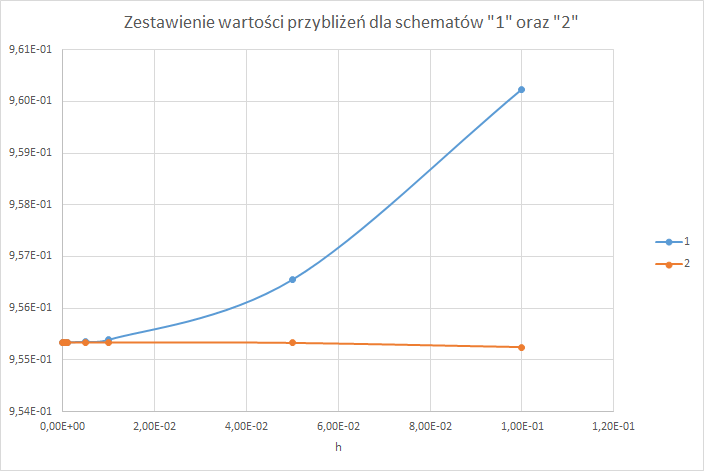
\includegraphics{Lab2/charts/wsp_e.png}
\newpage











